\documentclass[conference]{IEEEtran} 
%\usepackage{babel}
\IEEEoverridecommandlockouts
% The preceding line is only needed to identify funding in the first footnote. If that is unneeded, please comment it out.
\usepackage{cite}
\usepackage{amsmath,amssymb,amsfonts}
\usepackage{algorithmic}
\usepackage{graphicx}
\usepackage{textcomp}
\usepackage{xcolor}
\def\BibTeX{{\rm B\kern-.05em{\sc i\kern-.025em b}\kern-.08em
    T\kern-.1667em\lower.7ex\hbox{E}\kern-.125emX}}
\usepackage{hyperref}
\usepackage[space]{grffile}
\usepackage[margin=2.5cm]{geometry}
\usepackage{pdfpages}
%\usepackage{graphicx}
\usepackage[capitalize,noabbrev]{cleveref}

%\documentclass[a4paper]{paper} 
%\usepackage{babel}
%\usepackage{hyperref}
%\usepackage{amsfonts}
%\usepackage{amsmath}
%\usepackage{graphicx}
%\usepackage[space]{grffile}
%\usepackage[margin=2.5cm]{geometry}
%\usepackage{pdfpages}
%\usepackage{graphicx}
%\usepackage[capitalize,noabbrev]{cleveref}

\graphicspath{{img/}}
\title{Lightning Network imbalance measure and proactive channel rebalancing algorithm}
%\title{Imbalance measure and proactive channel rebalancing algorithm for the Lightning Network}
\begin{document} 

\author{\IEEEauthorblockN{1\textsuperscript{st} Rene Pickhardt}
\IEEEauthorblockA{\textit{Department of Computer Science} \\
\textit{Norwegian University of Science and Technology}\\
Gj{\o}vik, Norway \\
rene.m.pickhardt@ntnu.no}
\and
\IEEEauthorblockN{2\textsuperscript{nd} Mariusz Nowostawski}
\IEEEauthorblockA{\textit{Department of Computer Science} \\
\textit{Norwegian University of Science and Technology}\\
Gj{\o}vik, Norway \\
mariusz.nowostawski@ntnu.no}
}

\maketitle
\begin{abstract}
Making a payment in a privacy-aware payment channel network can be achieved by trying out several payment paths until one succeeds.
With a large network, such as the Lightning Network, a completion of a single payment can take up to several minutes.
We introduce a network imbalance measure and formulate the optimization problem of improving the balance of the network as a sequence of rebalancing operations of the funds within the channels along circular paths within the network.
As the funds and balances of channels are not globally known, we introduce a greedy heuristic
that improves every node's local balance despite the uncertainty.
In an empirical simulation on a snapshot of the Lightning Network we demonstrate that the imbalance distribution of the network has a Kolmogorov-Smirnoff distance of $0.74$ in comparison to the imbalance distribution after the heuristic is applied.
We further show that the success rate of a single unit payment increases from $11.2\%$ on the imbalanced network to $98.3\%$ in the balanced network.
Similarly, the median possible payment size across all pairs of participants increases from $0$ to $0.5$ mBTC for initial routing attempts on the cheapest possible path.
Executing $4$ different strategies for selecting rebalancing cycles lead to similar results 
indicating that a collaborative approach within the friend of a friend network might be preferable from a practical point of view.\footnote{A full version of this text - including a discussion about fee free rebalancing - is available at: \url{https://arxiv.org/abs/1912.09555}}

\end{abstract}
\begin{IEEEkeywords}
imbalance, rebalancing, optimization, Bitcoin, Lightning Network, payment channel networks, path finding, routing, liquidity, flow control, congestion control, game theory, uncertainty, simulations, collaborative problem solving, privacy 
\end{IEEEkeywords}

%==========================================================================
\section{Introduction}
The Lightning Network has been introduced in order to mitigate the scaling issues of blockchain technologies such as Bitcoin\cite{poon2016bitcoin} by creating a network of payment channels.
In order to protect users privacy while routing a payment through several payment channels privacy a payment network can use a source-based onion routing scheme, like the Sphinx Mix format~\cite{danezis2009sphinx}.
While the Lightning Network, for example, shares the capacity of public channels with its participants through its gossip protocol, the local split of the capacity of the channels into the balance of its participants is not shared with the rest of the network for two reasons:
(1) this would compromise the privacy as one could collect all changes of the channel balances and reconstruct the flow of payments;
(2) propagating this information would essentially mean that every node in the network is made aware of every payment which would have the same poor scaling properties as blockchain technology and other broadcast networks.
The decision to use source-based routing together with the unknown channel balances of the network results in a challenge for finding a path of payment channels so that all channels along the path have enough liquidity to be able to forward an attempted payment.
Currently, this challenge is met by probing paths until one succeeds.
It has been demonstrated that probing for paths can take more than 3 minutes for more than $5\%$ of the attempted payments~\cite{decker2019lnconf}. This leads to a poor payment latency and poor user experience.
Imagine a grocery store in which for every $20^{th}$ customer the cash register would have to wait three minutes until the payment was received.

This study examins the consequences of nodes proactively and collaboratively distributing their funds evenly across their channels.
We introduce the notation of an imbalanced network.
The imbalance is measured as the average of the imbalance scores of its nodes.
The node's imbalance of payment channels is defined as the Gini coefficient of a node's channel balance coefficients which are the relative amount of funds a node owns in a channel in comparison to the capacity of that channel.
Nodes can reduce their imbalance either by initiating a rebalancing their own channels themselves, or, by collaboratively rebalancing the channels with the help of their channel partners by conducting circular payments.

We formulate an optimization problem of finding a sequence of rebalancing operations that minimize the network's imbalance.
As the information necessary to solve the optimization problem is not publicly known in privacy-aware payment channel networks, we provide a greedy heuristic for its participants to find a minimum for the problem. 
In an empirical study, we show that the greedy heuristic will lead to a success rate of $98.3\%$ for a small payment between two arbitrary selected nodes.
Also the median possible payment size between all pairs of nodes increases from $0$ in the imbalanced network to $0.5$ mBTC in the best balanced networks that we found.

Looking at different strategies of finding rebalancing cycles we suggest, for the sake of speed, that nodes share with their neighbors on which local channels they would like to have inbound or outbound capacity.
This information could easily be probed anyway and will not to worsen the privacy of the nodes involved in rebalancing.

%==========================================================================
\section{Related Work}
\label{sec:relatedWork}

While the Lightning Network white paper~\cite{poon2016bitcoin} does not discuss path finding and states routing as an easy problem it is generally recognized that pathfinding on the Lightning Network is a difficult problem~\cite{piatkivskyi2018split, prihodko2016flare, bagaria2019boomerang, pickhardt2019pathfinding, grunspan2018ant, sivaraman2018routing}.
There is already research conducted in the field of rebalancing channels~\cite{khalil2017revive},which was about the cryptographic protocols used to make sure that participants can enforce the rebalancing that was agreed upon.
There are rebalancing operations for existing lightning implementations: c-lightning\footnote{\url{https://github.com/lightningd/plugins/tree/master/rebalance}} and for lnd\footnote{\url{https://github.com/bitromortac/lndmanage}}.
In particular, the idea of just in time rebalancing while fulfilling routing requests~\cite{pickhardt2019jit} has been implemented as JIT-routing for c-lightning\footnote{\url{https://github.com/lightningd/plugins/pull/66}}. 

% ===========================================================================
\section{Formalization and Assumptions}
\label{sec:formalization}

Let $N=(V,E,c)$ be a payment channel network with a finite set of nodes.
The payment channels are the edges in the network such that $E\subset V\times V$.
Additionally, we have a publicly known capacity function $c: E\longrightarrow \mathbb{N}$ that assigns a capacity to every edge of the network.
For every edge $e=(u,v)$ we denote $e_u:=(e,u)$ as the first participant of the channel and $e_v=(e,v)$ as the second participant.
Naturally, the capacity of every channel $e=(u,v)$ is privately split into the local balances with the balance function $b: E\times V\longrightarrow\mathbb{N}$ such that $b(e_u)+b(e_v)\stackrel{!}{=}c(e)$.

We define the channel balance coefficient for $u$ on the channel $e=(u,v)$ as  $\zeta_{(u,v)} = \frac{b(e_u)}{c(e)}$.
This is just the relative amount of funds that the participant $u$ has in the channel $e$.
In general, for an imbalanced chanel we have $\zeta_{(u,v)} \neq \zeta_{(v,u)}$.

The neighbor function $n : V \longrightarrow 2^{E}$ assigns every node a set of all the channels it is part of.
We call $U:=n(u)$ the neighborhood of node $u$.

The total funds of a participant $u$ are denoted as $\tau_u:=\displaystyle{\sum_{e\in U}b(e_u)}$.
The value of $\tau_u$ is constant while no payments are made and no channels are being opened and closed.
The balance function $b$ can vary.
The total capacity of a participant $u$ is denoted as $\kappa_u:=\displaystyle{\sum_{e\in U}c(e)}$.
Using the last two definitions let us define the node balance coefficient for a participant $u$ as $\nu_u = \frac{\tau_u}{\kappa_u}$.

We call a node $u$ {\bf balanced} if its channel balance coefficients $\zeta_{(u,v_1)},\dots,\zeta_{(u,v_d)}$ have the same value.\footnote{This value does not have to take a value of $0.5$, but it certainly is a reasonable goal.}
Consequently, we consider a node {\bf unbalanced}, if its local channel balance coefficients are unequal.
Statistically, inequality of a distribution can be measured with the Gini coefficient.
Thus, for a node $u$ with channel balance coefficients $\zeta_{(u,v_1)},\dots,\zeta_{(u,v_d)}$ we define $G_u = \frac{\displaystyle{\sum_{i\in U} \sum_{j \in U}} | \zeta_i - \zeta_j |}{2 \displaystyle{\sum_{i \in U} \sum_{j \in U} \zeta_j}}$.
If $G_u = 0$ this means that the channel balance coefficients are equal.
This value will be exactly the same as the node's balance coefficient $\nu_u$.
In contrast, if $G_u = 1$ the channel balance coefficients are distributed in the most unequal way.

Finally, $G$ denotes the imbalance of the network $G = \displaystyle{\frac{1}{|V|}\sum_{v\in V}G_v}$. It is the mean of the imbalance values of all nodes in the network.
A perfectly balanced network would be achieved if $G$ takes the value of $0$ whereas the balance is poor if the value of $G$ is close to 1.
Our goal is to find a balance function $b$ which minimizes $G$ given a privacy aware payment channel network with initial distribution of funds $\tau_{u_1},\dots,\tau_{u_n}$.
The constraint to this optimization problem is that the total funds $\tau_u$ are fixed for every node $u \in V$ and any choice of the balance function $b$.
As we lack knowledge about the global network state, we cannot apply standard optimization techniques such as gradient descent, conjugate gradient methods or simulated annealing.
We suggest to use a greedy heuristic in which every participant executes some operations to improve its own balance which others support if it also improves their balance.

\subsection{Description of the rebalancing algorithm}
\label{sec:Greedy Rebalancing Heuristic}

Participants use the local knowledge and make local adjustments trying to solve the optimization problem of finding $b$ such that $G$ is minimized.
\begin{enumerate}
\item A node $u$ computes its node balance coefficient $\nu_u$.
\item $u$ then computes its channel balance coefficients $\zeta_{(u,v_1)},\dots,\zeta_{(u,v_d)}$.
\item All channels $e=(u,v_i)$ for which the channel balance coefficient is higher 
than its node balance coefficient, are selected as $C = \{(u,v_i) | \zeta_{(u,v_i)} - \nu_u\ > 0\}$.\footnote{
  Note, that we do not need to take absolute values as $u$ will only be able to initiate a rebalancing operation by sending money which means decreasing its channel balance coefficient of $\zeta_{(u,v_i)}$ towards $\nu_u$.}.
\item From the candidate set $C$ a random channel $e=(u,v)$ is selected.
\item Now the node searches for a circular payment to itself along $e=(u,v)$ by choosing a path $p = [v,x_1,\dots,x_n,u]$. The amount of that payment should decrease the value of $\zeta_{(u,v)}$ to that of $\nu_u$ and can be computed as $a = c(e)\cdot (\zeta_{(u,v)}-\nu_u)$. The end of the circle should be a channel $(x_n,u)$ for which the channel balance coefficient $\zeta_{(u,x_n)}$ is smaller than the node balance coefficient $\nu_u$.\footnote{In one of the experiments we weaken this strong criteria and show empirically that it makes sense to drop it for the benefit of easier path finding at the cost of small oscillations of the algorithm.}
\item The node conducts the payment if all the nodes on the path $p$ agree to participate. It could happen that some nodes will only participate with a value smaller than $a$. As this is already progress $u$ will accept the suggested amount instead of being stubborn. 
\item Repeat all steps as long as the local balance coefficients are not even enough and as long as paths are found.
\end{enumerate}

\section{Experimental Setup}
\label{sec:setup}

We evaluated $4$ different strategies for finding rebalancing cycles. \texttt{cycles4} tests all cycles of length $4$ or smaller. In the same way \texttt{cycle5} tests all cycles of length $5$ or smaller. \texttt{foaf} tests most cycles of the friend of a friend network.\footnote{This approximation is achieved by using \texttt{cycle4} as a cycle base as all cycles of length 4 and smaller certainly are part of the friend of a friend network.}
\texttt{mpp} is short for multi-path payments and uses the same heuristic as \texttt{foaf} but will only take a $20^{th}$ of the maximum possible amount for rebalancing operation since it is supposed to split the rebalancing over various cycles.
Our approximation for \texttt{foaf} and \texttt{mpp} explains why the final results for these two strategies are not entirely monotonic but oscillating a bit.

We conducted our experiment on a snapshot of the public Lightning Network from October 2019.
As channels are currently almost always opened by one side\footnote{Dual funded channels are not part of the protocol and no implementation is merged to any of the standard nodes} we randomly guessed who opened the channel by a coin flip and allocated the entire channel capacity to that node.
As a result the histogram of all node balance coefficients had a mode of $0.5$ which is plausible with this random process\footnote{We refer again to the long Version of this paper for more details.}.

After we randomly chose the founder of each channel we compute the largest strongly connected component to remove nodes which had the funds allocated in a way that would not allow any rebalancing.
The strongly connected component consists of $2707$ nodes and $24161$ edges.
The diameter of the strongly connected component had a value of 10.
Almost $40\%$ of shortest paths are longer than the cycles that our strategies have tested. 
This demonstrates that the single rebalancing operations which we conducted were not covering the entire network but only taking place within local parts of the network.
This is particularly true for the rebalancing in the friend of a friend network.

In order to conduct the experiments we simulated the proposed algorithm and strategies in the following way.
For each channel we computed up to $5000$ rebalancing cycles following the defined strategy.
The number $5000$ was chosen to be as large as possible so that we were able to conduct the simulation on the $16$ GB of main memory of our machine.

% ==========================================================
\section{Results}
\label{sec:results}

\begin{figure}
 \centering
 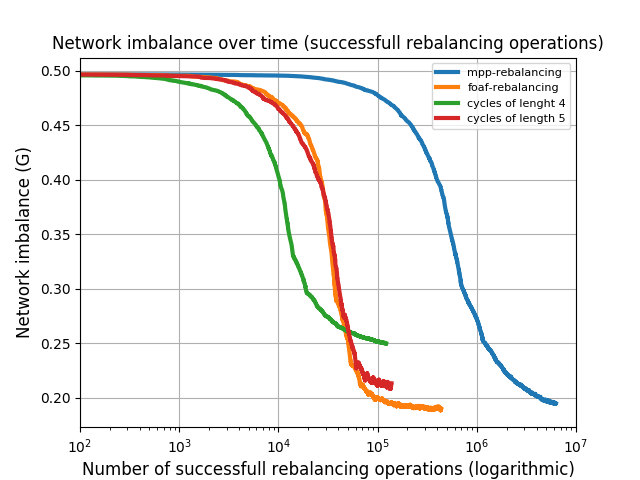
\includegraphics[width=6cm]{code/vs/fig/imba_vs_steps.png}
 \caption{Comparing how the imbalance score of the network behaves with the amount of successfull rebalancing operations. As the rebalancing amounts are much smaller with multi path payments the x-axis has a logarithmic scale.}
 \label{fig:imbalancehovertime}
\end{figure}

\cref{fig:imbalancehovertime} confirms that the imbalance of the network is decreasing over time when running our simulation.
This means that the network is becoming more balanced.
We see that most improvement is happening quite fast with $10$k to $100$k rebalancing operations being necessary.
This is not more than $37$ rebalancing operations per node.
Taking into account that the average node degree is $9$ this means that on average each node needs to successfully execute about $4$ rebalancing operations per channel.  
This seams plausible in the sense that every channel gets rebalanced at least once.\footnote{Note, that due to the collaborative behaviour of nodes a node might also get its channels rebalanced in the rebalancing attempts of other nodes.}
The multi-path rebalancing needs more operations which makes sense as we only rebalanced for a $20^{th}$ of the possible amount in the multi-path case since we wanted to have multiple other cycles to rebalance that particular channel.
While \texttt{cycle4} improves the balance more quickly, it does not reach the minimum imbalance as well as the other strategies.
In particular, the algorithm converges to a local minimum rather quickly.
Our experimental runs resulted in states that are not identical when we shuffled the order of cycles that we probed, however, the differences were negligible. 
We guess that the local minimum might be close to global minimum of the optimization problem.

\begin{figure}
 \centering
 
\includegraphics[width=6cm]{code/vs/fig/imba_vs_success_rates.png}
 \caption{Every time the imbalance score reached a new low to a two digit decimal we computed the probability for a random payment of the smallest possible amount to succeed on the cheapest path.}
 \label{fig:imba_vs_success}
\end{figure}

In~\cref{fig:imba_vs_success} we see that a lower imbalance score $G$ yields a higher success rate of payments as one would expect.
The success rate is measured by attempting a payment of $1$ Satoshi between all pairs of nodes and counting the relative amount of payment attempts for which the cheapest path from the source to the destination was successful.
We computed the success rate of every time the balance score hits a new score rounded to two decimals.
It is the first experiment that indicates that the defined imbalance score was well chosen. 
Again the multi-path payment strategy sticks out as it achieves a rather high success rate while the network is still rather imbalanced.
A success rate of $80\%$ is reached for an imbalance score of $0.43$.
Comparing this to~\cref{fig:imbalancehovertime} we see that about $250$k rebalance operations are necessary to achieve this success rate.
Even the worst performing algorithm achieves this success rate with far less than $100$k rebalancing operations and a much better overall imbalance score. 

This effect, while expected as multi-path rebalancing uses smaller amounts, is more pronounced in the next experiment.
As $1$ Satoshi payments are not too useful in a real world setting we checked if the overall amounts that can be routed increase in a better balanced network.

\begin{figure}
 \centering
 
\includegraphics[width=6cm]{code/vs/fig/imba_vs_median_payment_size.png}
 \caption{The imbalance of the network is plotted against the median value of payments that can be fulfilled between all pairs of nodes on the first attempt along the cheapest path. Note that failed payments are part of the statistics and counted as payments which can send $0$ Satoshi.}
 \label{fig:imba_vs_payment_size}
\end{figure}


In~\cref{fig:imba_vs_payment_size} we compare the imbalance of the network with the median possible payment amount which is computed as follows:
For all pairs of shortest paths on the base fee graph we look at the amount that could be forwarded along that path.
Finally we take the median of those values.
This means that at least $50\%$ of payment pairs are able to forward this amount.
Again we see that the lower the imbalance score becomes the higher the median possible payment size gets.
This suggests that statistically a more balanced network is able to successfully route higher payment amounts on the first try.
All four strategies are achieving a median possible payment amount of roughly $50000$ Satoshi.
This means that in a balanced network $50\%$ of payment pairs are able to successfully conduct a payment of $0.5$ mBTC along the cheapest path. 
The result also indicates that the strategy for probing rebalancing cycles seems to have little to no impact to the final abilities of the network to perform payments.


\begin{figure}
 \centering
 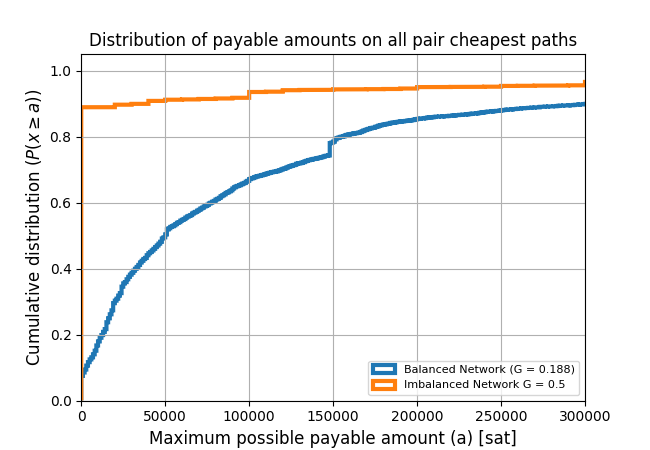
\includegraphics[width=6cm]{code/vs/fig/maximum_payable_amount_all_pair_chepest_paths_balanced_network.png}
 \caption{The maximal payable amounts on all pairs of cheapest paths on the initial imbalanced network and on the network after applying the friend of a friend rebalancing strategy.}
 \label{fig:cdf_paymentsize}
\end{figure}

We look a little bit closer at the data point of the most balanced network with the friend of a friend strategy and compare it to the imbalanced network.
Instead of only looking at the median we study the cumulative distribution function of the histogram in~\cref{fig:cdf_paymentsize}.
We can see that in the imbalanced network almost $88.8\%$ of the paths are not able to forward a single Satoshi (meaning a $11.2\%$ success rate).
This number drops below $1.7\%$ (meaning a $98.3\%$ success rate) for the balanced network.

For the friend of a friend network we examine the distribution of Gini coefficients with the initial distribution of Gini coefficients.
We provide the cumulative distribution function of both distributions with in~\cref{fig:cdf_gini}.

\begin{figure}
 \centering
 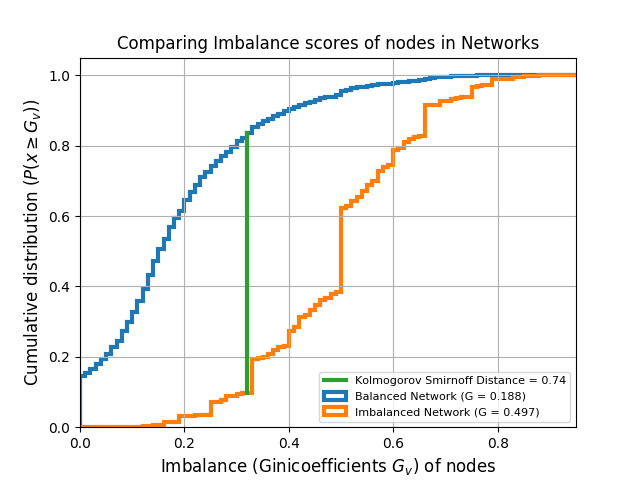
\includegraphics[width=6cm]{code/vs/fig/comparison distribution of Ginicoefficients.png}
 \caption{Comparing the distribution of the node's Gini coefficients before and after rebalancing with the friend of a friend strategy.}
 \label{fig:cdf_gini}
 \end{figure}

The Kolmogorov-Smirnoff distance reaches a value of $0.74$.
This verifies the statistical significance of the rebalancing heuristic in comparison to staying with the imbalanced network.
The median value of the Gini coefficients in the best balanced network we could acquire is about $0.15$.
In comparison, on the imbalanced network the median Gini coefficient is $0.5$.

Our results show that nodes do not need to strive for $\nu_u = 0.5$ and perfect local balance of their channels in order to produce high success rate of random payments.

% =========================================================================================
\section{Future Work}
\label{sec:future}

As the simulation had consumed a lot of computational resources, we have not check if the greedy heuristic is stable under concurrent payments and rebalancing operations taking place.
In a similar gist simulations on larger networks would be interesting but require more significant computational resources and time to be conducted.

The current experiments have assumed a stable network topology. 
However, every channel opening or closure, as well as every single payment, will change the imbalance of the network.
It is therefore necessary to study how it adapts if the topology changes in real time due to opening or closing channels as well as a reallocation of funds due to payments that are taking place.
In particular, it would be interesting to see how this heuristic works in combination with JIT-Routing as this would unbalance nodes to provide liquidity which our heuristic would then redistribute over the friend of a friend network.
This would occur along all nodes on a path in intersecting friend of a friend networks.
It would be interesting to see how this algorithm behaves together with Atomic Multipath Payments which are in the style of~\cite{bagaria2019boomerang} redundant but along our results carry at most $50000$ Satoshi. 


% =======================================================================
\section{Discussion}
\label{sec:conclusion}

Computing the rebalancing cycles is the most expensive operation in our simulation.
If the greedy heuristic is implemented in a real payment channel network, it would only be 
done locally by each node, which in itself is not expensive.
This holds true if those cycles will only be searched within the friend of a friend network which is typically small.
As the results of the different strategies for finding cycles did not vary and for the previous reason we propose to stick to rebalancing in the friend of a friend network and introducing a communications protocol between nodes to collaboratively find such rebalancing cycles by sharing some information.


% ==========================================================================================
\section{Acknowledgements}
\label{sec:ack}

We are grateful to Vivek Bagaria and Joachim Neu for an interesting discussion about their and our work that initiated this research. We thank Stefan Richter for helpful comments on early drafts of this work. A special thank goes to Thomas Gottron, Christian Decker and Dmytro Piatkivskyi. 
Finally we thank the donors to \url{https://tallyco.in/s/lnbook} and Patreons supporting open knowledge. 


\bibliography{lightningNetworkHealth}
\bibliographystyle{plain}

\end {document}
